\documentclass{standalone}
\usepackage{tikz}
\usetikzlibrary{patterns, positioning}


\begin{document}
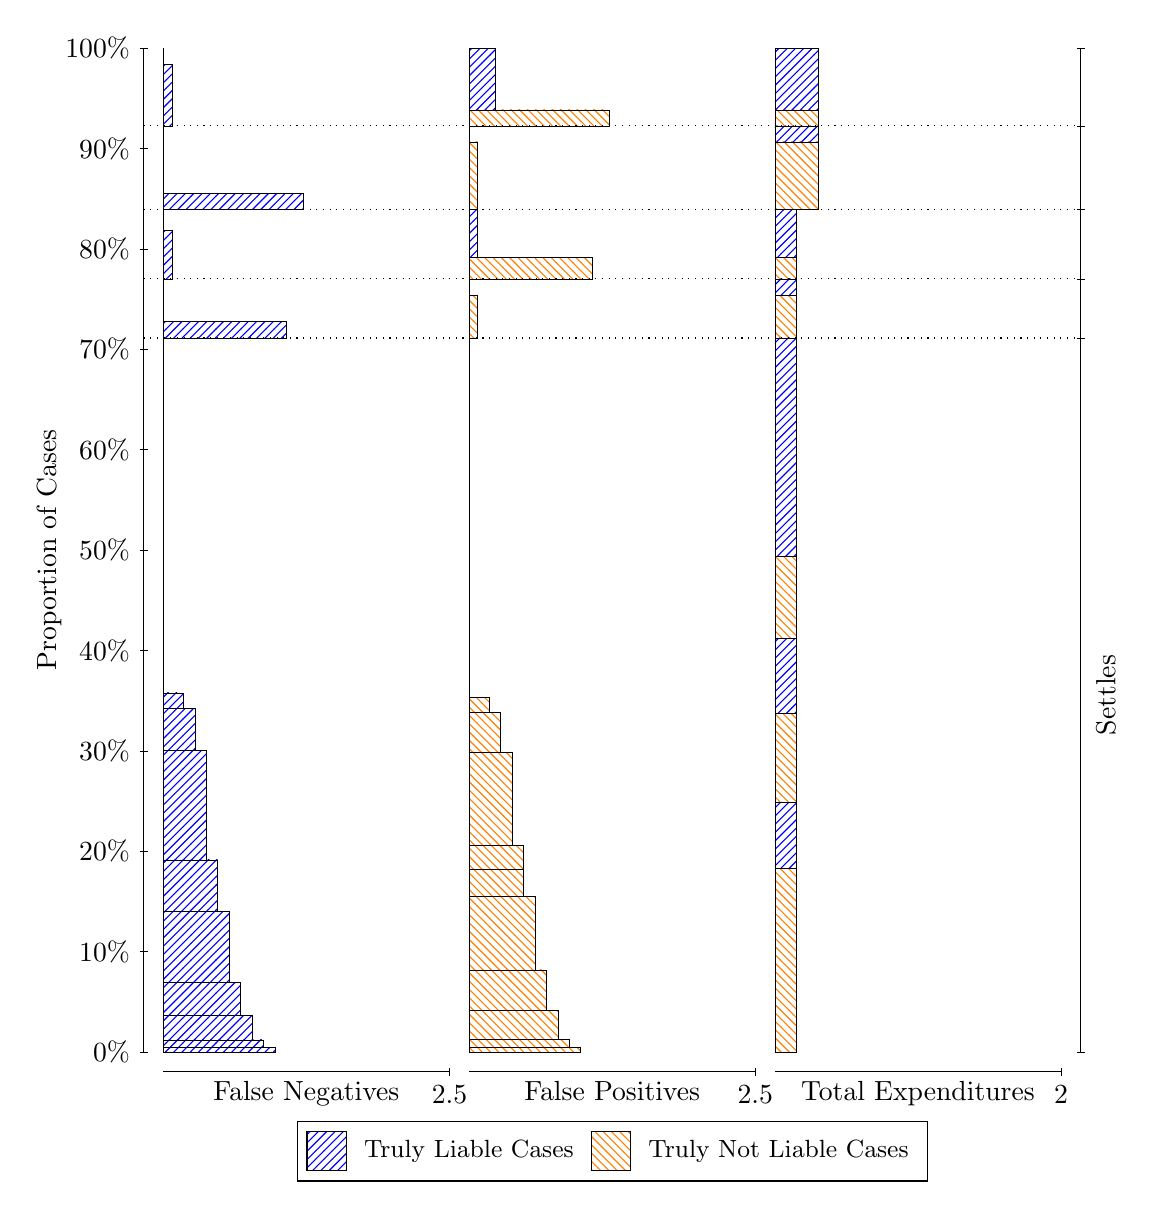
\begin{tikzpicture}
\draw[black, very thin] (1.5,1.75) -- (1.5,14.5);
\node[rotate=90, text=black, anchor=center] at (0.3, 8.125) {Proportion of Cases};
\draw[black, very thin] (1.45,1.75) -- (1.55,1.75);
\node[text=black, anchor=east] at (1.45, 1.75) {0\%};
\draw[black, very thin] (1.45,3.025) -- (1.55,3.025);
\node[text=black, anchor=east] at (1.45, 3.025) {10\%};
\draw[black, very thin] (1.45,4.3) -- (1.55,4.3);
\node[text=black, anchor=east] at (1.45, 4.3) {20\%};
\draw[black, very thin] (1.45,5.575) -- (1.55,5.575);
\node[text=black, anchor=east] at (1.45, 5.575) {30\%};
\draw[black, very thin] (1.45,6.85) -- (1.55,6.85);
\node[text=black, anchor=east] at (1.45, 6.85) {40\%};
\draw[black, very thin] (1.45,8.125) -- (1.55,8.125);
\node[text=black, anchor=east] at (1.45, 8.125) {50\%};
\draw[black, very thin] (1.45,9.4) -- (1.55,9.4);
\node[text=black, anchor=east] at (1.45, 9.4) {60\%};
\draw[black, very thin] (1.45,10.675) -- (1.55,10.675);
\node[text=black, anchor=east] at (1.45, 10.675) {70\%};
\draw[black, very thin] (1.45,11.95) -- (1.55,11.95);
\node[text=black, anchor=east] at (1.45, 11.95) {80\%};
\draw[black, very thin] (1.45,13.225) -- (1.55,13.225);
\node[text=black, anchor=east] at (1.45, 13.225) {90\%};
\draw[black, very thin] (1.45,14.5) -- (1.55,14.5);
\node[text=black, anchor=east] at (1.45, 14.5) {100\%};

\draw[black, very thin] (13.4,1.75) -- (13.4,14.5);
\draw[black, very thin] (13.35,1.75) -- (13.45,1.75);
\node[anchor=west] at (13.35, 1.75) {};
\draw[black, very thin] (13.35,10.818) -- (13.45,10.818);
\node[anchor=west] at (13.35, 10.818) {};
\draw[black, very thin] (13.35,11.568) -- (13.45,11.568);
\node[anchor=west] at (13.35, 11.568) {};
\draw[black, very thin] (13.35,12.453) -- (13.45,12.453);
\node[anchor=west] at (13.35, 12.453) {};
\draw[black, very thin] (13.35,13.511) -- (13.45,13.511);
\node[anchor=west] at (13.35, 13.511) {};
\draw[black, very thin] (13.35,14.5) -- (13.45,14.5);
\node[anchor=west] at (13.35, 14.5) {};

\draw[black, very thin, pattern color=blue, pattern=north east lines] (1.75,1.75) rectangle (3.167,1.8041);
\draw[black, very thin, pattern color=blue, pattern=north east lines] (1.75,1.8041) rectangle (3.0217,1.9043);
\draw[black, very thin, pattern color=blue, pattern=north east lines] (1.75,1.9043) rectangle (2.8763,2.2114);
\draw[black, very thin, pattern color=blue, pattern=north east lines] (1.75,2.2114) rectangle (2.731,2.6387);
\draw[black, very thin, pattern color=blue, pattern=north east lines] (1.75,2.6387) rectangle (2.5857,3.5322);
\draw[black, very thin, pattern color=blue, pattern=north east lines] (1.75,3.5322) rectangle (2.4403,4.1904);
\draw[black, very thin, pattern color=blue, pattern=north east lines] (1.75,4.1904) rectangle (2.295,5.5794);
\draw[black, very thin, pattern color=blue, pattern=north east lines] (1.75,5.5794) rectangle (2.1497,6.1114);
\draw[black, very thin, pattern color=blue, pattern=north east lines] (1.75,6.1114) rectangle (2.0043,6.311);
\draw[black, very thin, pattern color=orange, pattern=north west lines] (1.75,6.311) rectangle (1.75,10.818);
\draw[black, very thin, pattern color=blue, pattern=north east lines] (1.75,10.818) rectangle (3.3123,11.028);
\draw[black, very thin, pattern color=orange, pattern=north west lines] (1.75,11.028) rectangle (1.75,11.568);
\draw[black, very thin, pattern color=blue, pattern=north east lines] (1.75,11.568) rectangle (1.859,12.182);
\draw[black, very thin, pattern color=orange, pattern=north west lines] (1.75,12.182) rectangle (1.75,12.453);
\draw[black, very thin, pattern color=blue, pattern=north east lines] (1.75,12.453) rectangle (3.5303,12.656);
\draw[black, very thin, pattern color=orange, pattern=north west lines] (1.75,12.656) rectangle (1.75,13.511);
\draw[black, very thin, pattern color=blue, pattern=north east lines] (1.75,13.511) rectangle (1.859,14.297);
\draw[black, very thin, pattern color=orange, pattern=north west lines] (1.75,14.297) rectangle (1.75,14.5);
\draw[black, very thin, pattern color=orange, pattern=north west lines] (5.6333,1.75) rectangle (7.0503,1.8057);
\draw[black, very thin, pattern color=orange, pattern=north west lines] (5.6333,1.8057) rectangle (6.905,1.9074);
\draw[black, very thin, pattern color=orange, pattern=north west lines] (5.6333,1.9074) rectangle (6.7597,2.2772);
\draw[black, very thin, pattern color=orange, pattern=north west lines] (5.6333,2.2772) rectangle (6.6143,2.7917);
\draw[black, very thin, pattern color=orange, pattern=north west lines] (5.6333,2.7917) rectangle (6.469,3.7296);
\draw[black, very thin, pattern color=orange, pattern=north west lines] (5.6333,3.7296) rectangle (6.3237,4.064);
\draw[black, very thin, pattern color=orange, pattern=north west lines] (5.6333,4.064) rectangle (6.3237,4.3763);
\draw[black, very thin, pattern color=orange, pattern=north west lines] (5.6333,4.3763) rectangle (6.1783,5.5591);
\draw[black, very thin, pattern color=orange, pattern=north west lines] (5.6333,5.5591) rectangle (6.033,6.0612);
\draw[black, very thin, pattern color=orange, pattern=north west lines] (5.6333,6.0612) rectangle (5.8877,6.2572);
\draw[black, very thin, pattern color=blue, pattern=north east lines] (5.6333,6.2572) rectangle (5.6333,10.818);
\draw[black, very thin, pattern color=orange, pattern=north west lines] (5.6333,10.818) rectangle (5.7423,11.358);
\draw[black, very thin, pattern color=blue, pattern=north east lines] (5.6333,11.358) rectangle (5.6333,11.568);
\draw[black, very thin, pattern color=orange, pattern=north west lines] (5.6333,11.568) rectangle (7.1957,11.839);
\draw[black, very thin, pattern color=blue, pattern=north east lines] (5.6333,11.839) rectangle (5.7423,12.453);
\draw[black, very thin, pattern color=orange, pattern=north west lines] (5.6333,12.453) rectangle (5.7423,13.307);
\draw[black, very thin, pattern color=blue, pattern=north east lines] (5.6333,13.307) rectangle (5.6333,13.511);
\draw[black, very thin, pattern color=orange, pattern=north west lines] (5.6333,13.511) rectangle (7.4137,13.714);
\draw[black, very thin, pattern color=blue, pattern=north east lines] (5.6333,13.714) rectangle (5.9603,14.5);
\draw[black, very thin, pattern color=orange, pattern=north west lines] (9.5167,1.75) rectangle (9.7892,4.0816);
\draw[black, very thin, pattern color=blue, pattern=north east lines] (9.5167,4.0816) rectangle (9.7892,4.9162);
\draw[black, very thin, pattern color=orange, pattern=north west lines] (9.5167,4.9162) rectangle (9.7892,6.0501);
\draw[black, very thin, pattern color=blue, pattern=north east lines] (9.5167,6.0501) rectangle (9.7892,6.9977);
\draw[black, very thin, pattern color=orange, pattern=north west lines] (9.5167,6.9977) rectangle (9.7892,8.0394);
\draw[black, very thin, pattern color=blue, pattern=north east lines] (9.5167,8.0394) rectangle (9.7892,10.818);
\draw[black, very thin, pattern color=orange, pattern=north west lines] (9.5167,10.818) rectangle (9.7892,11.358);
\draw[black, very thin, pattern color=blue, pattern=north east lines] (9.5167,11.358) rectangle (9.7892,11.568);
\draw[black, very thin, pattern color=orange, pattern=north west lines] (9.5167,11.568) rectangle (9.7892,11.839);
\draw[black, very thin, pattern color=blue, pattern=north east lines] (9.5167,11.839) rectangle (9.7892,12.453);
\draw[black, very thin, pattern color=orange, pattern=north west lines] (9.5167,12.453) rectangle (10.062,13.307);
\draw[black, very thin, pattern color=blue, pattern=north east lines] (9.5167,13.307) rectangle (10.062,13.511);
\draw[black, very thin, pattern color=orange, pattern=north west lines] (9.5167,13.511) rectangle (10.062,13.714);
\draw[black, very thin, pattern color=blue, pattern=north east lines] (9.5167,13.714) rectangle (10.062,14.5);
\draw[black, dotted] (1.5,10.818) -- (13.4,10.818);
\draw[black, dotted] (1.5,11.568) -- (13.4,11.568);
\draw[black, dotted] (1.5,12.453) -- (13.4,12.453);
\draw[black, dotted] (1.5,13.511) -- (13.4,13.511);
\draw[black, very thin] (1.75,1.5) -- (5.3833,1.5);
\node[text=black, anchor=north] at (3.5667, 1.5) {False Negatives};
\draw[black, very thin] (5.3833,1.45) -- (5.3833,1.55);
\node[text=black, anchor=north] at (5.3833, 1.45) {2.5};

\draw[black, very thin] (5.6333,1.5) -- (9.2667,1.5);
\node[text=black, anchor=north] at (7.45, 1.5) {False Positives};
\draw[black, very thin] (9.2667,1.45) -- (9.2667,1.55);
\node[text=black, anchor=north] at (9.2667, 1.45) {2.5};

\draw[black, very thin] (9.5167,1.5) -- (13.15,1.5);
\node[text=black, anchor=north] at (11.333, 1.5) {Total Expenditures};
\draw[black, very thin] (13.15,1.45) -- (13.15,1.55);
\node[text=black, anchor=north] at (13.15, 1.45) {2};

\node[text=black, centered, rotate=90] at (13.72, 6.2841) {Settles};





\draw (7.449999999999999,1.5) node[draw=none] (baseCoordinate) {};
\begin{scope}[align=center]
        \matrix[scale=0.5, draw=black, below=0.5cm of baseCoordinate, nodes={draw}, column sep=0.1cm]{
            \node[rectangle, draw, minimum width=0.5cm, minimum height=0.5cm, pattern color=blue, pattern=north east lines] {}; &
            \node[draw=none, font=\small, text=black] (B) {Truly Liable Cases}; &
            \node[rectangle, draw, minimum width=0.5cm, minimum height=0.5cm, pattern color=orange, pattern=north west lines] {}; &
            \node[draw=none, font=\small, text=black] (B) {Truly Not Liable Cases}; \\
            };
\end{scope}

\end{tikzpicture}
\end{document}